% ===========================================================================
% Appendix D. Corrections relative to the shipped release, and reconciliation
% Sources: git log of branch fix/allied-base-paper (audit commits 7003d11 ... 3eb9240 and the
% later data and method commits up to 3122cea), the audit's fix logs, README changelog, and the
% corrected code in R/, scripts/, config/. Reconciliation numbers: paper/results/reconcile.json
% (scripts/paper/fig_reconcile.R), shipped release of 3 September 2026 against the final run of
% 12 October 2026 (network at lambda = 0.78). Item detail: Online Appendix oa:corrections.
% ===========================================================================
\section{Corrections relative to the shipped release}
\label{app:corrections}

The indices were first released in September 2026. That \emph{shipped release} combined artefacts
built at different dates: the Energy Security and Economic Opportunity pillars and the Strategic
Index of 3~September 2026 rested on a policy component table of 6~February 2026, the partnership
tables dated from 24~March 2026 and the allied network outputs from 23~February 2026. Before the
results of this paper were produced, the pipeline was audited end to end, from the staged raw
inputs to the published tables, and every defect found was corrected. A set of data and method
changes followed, decided while the paper was written. All results in
Sections~\ref{sec:es}--\ref{sec:robustness} come from one complete run of the corrected pipeline,
the final run of 12~October 2026, built from a single revision of the code. This appendix lists
every correction and change and compares the shipped release with the final one, so that a reader
who holds numbers from the shipped release can tell which changed and why.

% ---------------------------------------------------------------------------
\subsection{Scope and kinds of change}
\label{subsec:corr_scope}

Table~\ref{tab:corrections_index} gives one line per item. The items coded A to N are defects.
They fall into three kinds. \emph{Input defects} change what a variable measures: a join on
mismatched keys, a wrong supply-chain stage, a ranking taken over the wrong population.
\emph{Aggregation defects} change how correctly measured variables are combined: an unobserved
category scored as zero, a row counted several times. \emph{Reporting defects} leave every value
unchanged but misstate a diagnostic, a label or the documentation. The distinction matters for
reconciliation: reporting defects change no number, aggregation defects mostly shift the levels of
whole cells, and input defects can reorder countries within a cell. The uncertainty and sensitivity
analyses recommended for composite indicators vary weights, normalisation and aggregation for given
inputs \citep{saisana2005uncertainty,oecd2008handbook}; they can reveal the second kind of defect
but not the first, which is why the audit traced each variable from its source to the index.

The items coded D (data) and M (method) are not defects. They are changes of source, basket or
design adopted after the audit, most of them by explicit decision, and they are described in the
main text where they apply. For each defect the audit re-ran the affected builders on the inputs
saved with the shipped release and compared the outputs. These \emph{pre-rerun effects}, reported
in Online Appendix~\ref{oa:corrections} with the symptom and the correction of each item, isolate
one correction on inputs that still embed the others; they are not results of the paper. Each
correction comes with unit tests that encode the corrected behaviour, and the code in \texttt{R/},
\texttt{scripts/} and \texttt{config/} is its specification.

{\small
\setlength{\LTcapwidth}{\textwidth}
\begin{longtable}{@{}p{0.35in}p{2.85in}p{0.8in}p{1.35in}p{0.42in}@{}}
  \caption{Index of corrections and changes relative to the shipped release}\label{tab:corrections_index}\\
  \toprule
  Item & Correction or change & Commit & Outputs affected & Status \\
  \midrule
  \endfirsthead
  \multicolumn{5}{@{}l}{\emph{Table~\ref{tab:corrections_index}, continued}}\\
  \toprule
  Item & Correction or change & Commit & Outputs affected & Status \\
  \midrule
  \endhead
  \midrule
  \multicolumn{5}{r@{}}{\emph{continued on next page}}\\
  \endfoot
  \bottomrule
  \multicolumn{5}{@{}p{\textwidth}@{}}{\footnotesize\emph{Notes:} Status R: the defect changed
  values in the shipped release. L: latent; it did not change the shipped release but would have
  changed a rerun. D: diagnostics, labels or documentation only. X: change of data or method adopted
  after the audit, not a defect. Commits are on branch \texttt{fix/allied-base-paper}; the audit
  corrections (\texttt{7003d11} to \texttt{cd3b6cc}) were applied to revision \texttt{c0cd1ce}.
  Item detail: Online Appendix~\ref{oa:corrections}.}\\
  \endlastfoot
  \multicolumn{5}{@{}l}{\emph{Aggregation}}\\
  A1 & Available-case aggregation: an unobserved category no longer counts as zero & \texttt{7003d11} & ES, EO, PSI & R \\
  A2 & Imputation only in groups with an observed country & \texttt{7003d11} & ES, EO & L \\
  A3 & Imputed flag for groups with several components & \texttt{7003d11} & ES, EO diagnostics & D \\
  A4 & Energy Prices scored; guards for unproduced score variables & \texttt{7003d11}, \texttt{cd3b6cc} & ES, EO Upstream & R \\
  A5 & Orphan EO Reserves weight and 88 phantom EO cells removed & \texttt{7003d11} & EO & R \\
  A6 & Contribution tables reconcile to the index & \texttt{7003d11} & decompositions & D \\
  A7 & Overall scores no longer collapse into one row & \texttt{7003d11} & ES, EO & L \\
  \multicolumn{5}{@{}l}{\emph{Country universe}}\\
  C1 & One canonical name per economy & \texttt{9a5a72a}, \texttt{c840032} & all & R \\
  C2 & Aggregates, residual and historical entities dropped & \texttt{9a5a72a} & all & R \\
  C3 & Comtrade vintages need at least 50 reporters & \texttt{9a5a72a} & ES Minerals Trade & L \\
  \multicolumn{5}{@{}l}{\emph{Energy Security and production themes}}\\
  E1 & Harmonised mineral names (graphite, rare earths) & \texttt{c840032} & mineral categories & R \\
  E2 & Refining assigned to the Midstream & \texttt{c840032} & ES Foreign Dependency & R \\
  E3 & Zero supply for non-suppliers, ranked below every supplier & \texttt{c840032} & ES Foreign Dependency & R \\
  E4 & Reserves roll-up over all of a technology's minerals & \texttt{c840032} & ES Reserves & R \\
  E5 & Wind consumption, within-technology growth, one regional value per country & \texttt{c840032} & ES, EO Consumption & R \\
  E6 & Minerals Trade scores market share and concentration & \texttt{c840032}, \texttt{cd3b6cc} & ES Minerals Trade & R \\
  E7 & Minerals investment split by demand; no manufactured zero cells & \texttt{c840032} & ES, EO Investment; SI & R \\
  E8 & Electrolyser capacity mapped to Green Hydrogen & \texttt{c840032} & EO Foreign Dependency & R \\
  E9 & Mineral production depth as a demand-weighted share of world mined supply & \texttt{c939ad6} & EO Production & R \\
  E10 & EV Midstream keeps the non-EU European economies & \texttt{c939ad6} & ES, EO EV Midstream & R \\
  E11 & Self-sufficiency and net-export ratios named for what they measure; ties & \texttt{c939ad6} & ES Energy Imports & R \\
  E12 & Absent EI production no longer read as zero (EIA fill, same-year pairing) & \texttt{cce8985}, \texttt{7f0190c} & ES Energy Imports, EO Production & R \\
  \multicolumn{5}{@{}l}{\emph{Trade and Economic Opportunity themes}}\\
  T1 & Separate ES and EO trade themes; ES deficit term computed & \texttt{fe605b6}, \texttt{cd3b6cc} & ES, EO Trade & R \\
  T2 & Export size and feasibility ranked across economies & \texttt{fe605b6} & EO Trade & R \\
  T3 & Market share as the share of the basket & \texttt{fe605b6} & ES, EO Trade & R \\
  T4 & HS6 crosswalk: raw materials, logs, duplicate keys & \texttt{fe605b6} & ES, EO Trade & R \\
  T5 & Legacy HS codes bridge the HS92 Atlas & \texttt{fe605b6} & ES, EO Trade & R \\
  T6 & Levelised cost counted once in Cost Competitiveness & \texttt{fe605b6}, \texttt{cd3b6cc} & EO Cost Competitiveness & R \\
  T7 & Technological readiness broadcast to economies & \texttt{fe605b6} & EO, SI & R \\
  T8 & Technology Demand counts each source once & \texttt{fe605b6}, \texttt{cd3b6cc} & EO Technology Demand & R \\
  T9 & Export-concentration index ranked over headline cells only & \texttt{23f20da} & ES, EO Trade & R \\
  T10 & Energy-trade file completed (60 basket codes, 13 reporters, Qatar's LNG) & \texttt{9778e34} & ES, EO Trade & R \\
  T11 & Unique demand keys; IEA 2035 shares over the world total incl.\ ``Other'' & \texttt{c939ad6} & EO Technology Demand & D \\
  T12 & Zero lending-rate stubs dropped (New Zealand) & \texttt{c939ad6} & EO Cost Competitiveness & R \\
  T13 & IMF price units and source labels & \texttt{c939ad6} & labels & D \\
  \multicolumn{5}{@{}l}{\emph{Policy and Strategic indices}}\\
  P1 & Separate jurisdiction weights for IEA PAMS and NIPO & \texttt{81ede9d} & Policy, SI & R \\
  P2 & Whole-word stage tagging of IEA policies & \texttt{81ede9d} & Policy, SI & R \\
  P3 & Policy coverage of Korea, the UAE, France, Italy and Denmark & \texttt{81ede9d} & Policy, SI, network & R \\
  P4 & Policy component table rebuilt with provenance & \texttt{81ede9d} & Policy, SI & R \\
  P5 & NIPO as-of date capped at the extract's last announcement & \texttt{81ede9d} & NIPO (robustness only) & R \\
  P6 & Security and security need stored under their own names in the SI & \texttt{81ede9d} & SI tables, charts & D \\
  P7 & No imputation of pillar or policy values in the SI & \texttt{81ede9d} & SI & R \\
  P8 & Sectors with a constant pillar detected and excluded & \texttt{81ede9d} & SI, allied pick & R \\
  P9 & Oil lifecycle emissions in the technology weight (SRREN median) & \texttt{6ef4831} & SI & R \\
  \multicolumn{5}{@{}l}{\emph{Bilateral indices}}\\
  B1 & Duplicated Friendshore rows and self-dyads removed & \texttt{45efcf2} & FS, PSI, network & R \\
  B2 & Outbound investment: three measures, name matching, missing vs zero & \texttt{45efcf2} & FS, PSI, network & R \\
  B3 & Development potential at partner level & \texttt{45efcf2} & DP, PSI, network & R \\
  B4 & Available-case PSI; partner identity by ISO3 code & \texttt{45efcf2} & PSI & R \\
  B5 & Direction conventions; headline technologies only & \texttt{45efcf2} & FS, PO, PSI, network & R \\
  \multicolumn{5}{@{}l}{\emph{Allied network}}\\
  N1 & Development join fan-out & \texttt{2eeb111} & network & R \\
  N2 & Duplicate edges and split country records & \texttt{2eeb111} & network & R \\
  N3 & Friendshore half of the edge oriented consumer to producer & \texttt{2eeb111} & network & R \\
  N4 & Selection and portfolio counts over distinct countries & \texttt{2eeb111} & network & R \\
  N5 & Coalition code of the United Arab Emirates & \texttt{2eeb111}, \texttt{81ede9d} & network, SI & R \\
  N6 & MILP threshold, solver reporting, greedy flows & \texttt{2eeb111} & network & R \\
  N7 & Missing node components and stages without signal & \texttt{2eeb111} & network & R \\
  \multicolumn{5}{@{}l}{\emph{Data changes}}\\
  D1 & Nuclear Upstream on Red Book uranium resources and production & \texttt{6d874a3} & ES, EO Nuclear Upstream & X \\
  D2 & Technological readiness mapped by stage (IEA Clean Technology Guide) & \texttt{fefbc37} & EO, SI & X \\
  D3 & All-reporter Comtrade dyads, importer first, else mirror $\times1.06$; Taiwan & \texttt{c8ca2d5} & trade, FS, PO, network & X \\
  D4 & HS6 basket review; electricity out of Electric Grid Upstream & \texttt{3f52711} & ES, EO Trade & X \\
  D5 & Copper and aluminium basket for Electric Grid Upstream & \texttt{0bbcf79} & ES, EO Trade & X \\
  D6 & Critical-mineral reserves from USGS MCS 2026 & \texttt{8ef7ab0} & ES Reserves, coalition & X \\
  D7 & HS 851762 out of Grid Midstream; Hong Kong out of export measures & \texttt{23f20da} & ES, EO Trade & X \\
  D8 & ILO earnings from a staged copy & \texttt{9776f9f} & EO Cost Competitiveness & X \\
  D9 & Upstream trade baskets for EV, Wind, Nuclear, Solar, Semiconductors & \texttt{0fc5b73} & ES, EO Trade & X \\
  D10 & CM-FDI investment ties and Chinese-parent exposure in Friendshore & \texttt{78be8b5} & FS, PSI, network & X \\
  \multicolumn{5}{@{}l}{\emph{Method changes}}\\
  M1 & Rankability rule: sovereign, at most half the weight imputed & \texttt{5f60417} & ES, EO, SI, PSI & X \\
  M2 & Coalition derived from UN voting, in two tiers; EU as one node & \texttt{07e1783}, \texttt{19bf99e} & SI picks, PSI, network & X \\
  M3 & Policy index: IEA PAMS required, CAT where rated; NIPO (robustness only, October 2026 run) and dual use out & \texttt{0aaf68d}, \texttt{aefd3ef} & Policy, SI & X \\
  M4 & Endowment screen for the allied pick & \texttt{0aaf68d} & allied pick & X \\
  M5 & Alignment in Friendshore; conduit centres out; core-view PSI & \texttt{6ef4831} & FS, PSI & X \\
  M6 & Network on Upstream and Midstream, diversification term, caps, no policy term & \texttt{5afe34c} & network & X \\
  M7 & Calibration rule for $\lambda$; $\lambda=0.78$ on the final inputs & \texttt{3122cea} & network & X \\
\end{longtable}
}

% ---------------------------------------------------------------------------
\subsection{The main corrections}
\label{subsec:corr_defects}

Four defects account for most of the difference between the releases, and each is stated here
formally. Write $c_{itsk}$ for the score of category $k$ in cell $(i,t,s)$, $w_k$ for its weight and
$R_{its}$ for the categories with a row for the cell, observed or not.

\emph{Unobserved categories as zeros (A1).} The shipped builder kept an unobserved category in
the denominator,
\begin{equation}\label{eq:corr_pillar_old}
  I^{\text{shipped}}_{its}=\frac{\sum_{k\in R_{its}} w_k\,c_{itsk}\,\1[c_{itsk}\ \text{observed}]}
  {\sum_{k\in R_{its}} w_k},
\end{equation}
so it counted as zero and a cell with no observed category scored zero. The corrected pillar is the
available-case mean,
\begin{equation}\label{eq:corr_pillar_new}
  I_{its}=\frac{\sum_{k\in R_{its}} w_k\,c_{itsk}\,\1[c_{itsk}\ \text{observed}]}
  {\sum_{k\in R_{its}} w_k\,\1[c_{itsk}\ \text{observed}]},
\end{equation}
and a cell without an observed category is missing (Section~\ref{sec:normalization}). Combined with
the zero cells that the investment theme manufactured (E7), the shipped rule made Energy Security
in Nuclear Upstream zero for every economy, so its security need was maximal everywhere and it was
the top allied pick of 8 of the 18 shipped allies.

\emph{Market share of a basket (T3).} The shipped trade theme averaged a country's product-level
world shares with its own exports as weights, which measures dominance in the products it ships
rather than weight in the basket:
\begin{equation}\label{eq:corr_share_old}
  \widetilde{ms}_{its}=\frac{\sum_{h\in B_{ts}}X_{ih}\,(X_{ih}/W_h)}{\sum_{h\in B_{ts}}X_{ih}},
  \qquad
  ms_{its}=\frac{\sum_{h\in B_{ts}}X_{ih}}{\sum_{h\in B_{ts}}W_h},
\end{equation}
with $X_{ih}$ exports of product $h$, $W_h$ world exports and $B_{ts}$ the basket. The corrected
measure is $ms_{its}$. In the shipped Batteries Midstream basket the Democratic Republic of the
Congo had $\widetilde{ms}=0.862$ against a basket share of 0.0074. Together with the ranking of
export size across economies rather than within each reporter (T2), the correction changes the ten
leading EO Trade scores in Batteries Midstream, on the shipped inputs, from ore exporters (Chile,
Peru, Zimbabwe) to cell and material manufacturers (China, Germany, the United States). The ES and
EO trade themes had, moreover, been identical tables (T1).

\emph{The PSI denominator (B4).} Development potential is defined only for partners that are not
high-income, but for a high-income partner it kept its weight and contributed nothing,
\begin{equation}\label{eq:corr_psi_old}
  \PSI^{\text{shipped}}_j=0.4\,C^{\FS}_j+0.4\,C^{\PO}_j\ \le\ 0.8 ,
\end{equation}
so high-income partners sat at the bottom: the United States ranked 185th of 218. With the
duplication of Friendshore rows (B1) and the outbound-investment defect (B2), the shipped PSI ordering
does not survive the corrections.

\emph{The network fan-out (N1).} The node table joined the dyadic development table without
aggregating it, and the greedy solver took the first rows of the ranked candidates rather than
distinct countries, so in the affected stages one country was selected with $k^2$ rows of share
$1/k$:
\begin{equation}\label{eq:corr_fanout}
  n_{\text{producers}}=k^2,\qquad \HHI=\sum_{r=1}^{k^2}\Big(\frac1k\Big)^2=1 .
\end{equation}
The shipped specialisation table had 606{,}866 rows, of which 2{,}339 were distinct. With the
transposed Friendshore half of the edge (N3), counts over rows (N4) and the invalid code for the
United Arab Emirates (N5), the shipped network outputs carry no usable information.

The remaining defects are smaller but not negligible. The country standardiser left 30 economies
under two or three spellings, each taking its own rank in every S-curve (C1); graphite and the rare
earths fell out of every mineral join (E1); refining was pooled with mining (E2); and the policy
block had not written its table since February 2026 (P4), with substring stage rules that tagged
37 percent of IEA policies Upstream (P2). Three latent defects (A2, A7, C3) would have changed a
rerun; A7 alone would have removed every category built from an overall score. Item E12 is a
defect found late: an economy without its own production row in the Energy Institute's tables
\citep{ei2026statistical} was read as producing nothing, so New Zealand counted as importing all its
gas. Its production now comes from the EIA \citep{eia2026international}.

% ---------------------------------------------------------------------------
\subsection{Data and method changes}
\label{subsec:corr_changes}

The data changes replace or extend sources. Nuclear Upstream, which the shipped release scored on a
manufactured zero and the audited code on the world uranium price alone, is scored on the identified
resources and mine production of the OECD-NEA/IAEA Red Book \citep{oecdnea2026uranium} (D1). Critical-mineral reserves come from the USGS
Mineral Commodity Summaries 2026 \citep{usgs2026mcs} rather than the older USGS figures repeated in
the Energy Institute's sheets (D6). Technological readiness is mapped by stage from the IEA Clean
Technology Guide \citep{iea2026cleantechguide} (D2). Bilateral trade comes from all-reporter
Comtrade dyads, importer report first, else the exporter's mirror declaration times 1.06 (D3). The
HS6 baskets were reviewed against a dominant-use rule, which removed 92 basket rows; electricity
left Electric Grid Upstream, which received a copper and aluminium input basket, telecommunications
switching equipment left Electric Grid Midstream, and five technologies received Upstream baskets
(D4, D5, D7, D9). Hong Kong left the Comtrade export measures as a re-export hub (D7). Friendshore
gained investment ties and a Chinese-parent exposure component from the CM-FDI project data
\citep{bandara2026cmfdi} (D10). One limitation of the sources remains: the IEA's 2035 announced
manufacturing-capacity shares are regional for Europe, so every EU member carries the EU's share in
the variables built on them (Section~\ref{subsec:discussion_limitations}).

The method changes are the rankability rule (M1); the coalition derived from UN-voting alignment in
two tiers, with the EU-27 as one network node (M2), which replaced the shipped hand-picked list of 23
economies; a Policy index built on IEA PAMS, combined with CAT where CAT rates the country, which
dropped the GTA NIPO component and the dual-use score of the shipped four-component index (M3; NIPO
survives only as a robustness variant, rebuilt from the October 2026 extract for 77 jurisdictions);
the endowment screen of the allied pick (M4); the alignment component, the exclusion of conduit
financial centres and the core-coalition view of the PSI (M5); and a network restricted to the
Upstream and Midstream stages, with a concave diversification term, GDP-log portfolio caps and no
policy term (M6). The diversification weight follows a rule rather than a number (M7): the smallest
$\lambda$ whose median designed Herfindahl index does not exceed the nodes' median observed export
Herfindahl index. Applied to successive input vintages, the rule gave 1.5 on the hand-picked list,
then 0.94 on 34 nodes, 0.92 on 36, 0.95 and 0.94 on 37 nodes with 14 basket stages, and 0.78 on the
final 37-node inputs with 18 basket stages; only the last is used in this paper.

% ---------------------------------------------------------------------------
\subsection{Reconciliation with the shipped release}
\label{subsec:corr_reconciliation}

\paragraph{Matching and coverage.} The comparison uses the headline tables of the two releases.
Every shipped country name is mapped to its canonical name (C1), units without an ISO3 code are
dropped (C2), and where two spellings give the same key the record under the canonical spelling is
kept. Harmonisation alone reduces the shipped Energy Security table from 270 strings to 237
economies, merging 162 rows of 29 economies that appeared under two or three spellings.
Table~\ref{tab:reconcile_coverage} reports the counts. Of the harmonised $\ES$ cells 5{,}522 are in
both releases; 710 are new in the final one, mostly economies reached by the rebuilt trade themes
and the Green Hydrogen Midstream cells the shipped $\ES$ did not score. For $\EO$, 6{,}598 cells are
in both and 533 are new, mostly imputed (median imputed weight share 0.68) and only 11 rankable.

\begin{table}[htbp]
  \centering
  \begin{threeparttable}
  \caption{Coverage of the headline tables: shipped and final release}
  \label{tab:reconcile_coverage}
  \small
  \begin{tabular}{@{}l r r@{}}
    \toprule
    & Shipped release & Final release \\
    \midrule
    \multicolumn{3}{@{}l}{\emph{Energy Security}} \\
    Rows (country--technology--stage cells) & 5{,}746 & 6{,}232 \\
    \quad rankable & -- & 4{,}163 \\
    Distinct country strings & 270 & 219 \\
    \quad non-country units dropped (rows) & 17 & -- \\
    \quad merged spellings (rows) & 162 & -- \\
    Economies after harmonisation & 237 & 219 \\
    Technology--stage pairs scored & 31 & 30 \\
    Cells in both releases & 5{,}522 & 5{,}522 \\
    \quad rankable in the final release & -- & 3{,}731 \\
    Cells in one release only & 45 & 710 \\
    \addlinespace
    \multicolumn{3}{@{}l}{\emph{Economic Opportunity}} \\
    Rows (country--technology--stage cells) & 6{,}923 & 7{,}131 \\
    \quad rankable & -- & 4{,}301 \\
    Distinct country strings & 272 & 219 \\
    \quad non-country units dropped (rows) & 56 & -- \\
    \quad merged spellings (rows) & 234 & -- \\
    Economies after harmonisation & 237 & 219 \\
    Technology--stage pairs scored & 33 & 33 \\
    Cells in both releases & 6{,}598 & 6{,}598 \\
    \quad rankable in the final release & -- & 4{,}290 \\
    Cells in one release only & 35 & 533 \\
    \addlinespace
    \multicolumn{3}{@{}l}{\emph{Strategic Index}} \\
    Scored cells & 571 & 3{,}154 \\
    Countries & 18 & 174 \\
    Sectors & 32 & 30 \\
    Cells in both releases & 477 & 477 \\
    \bottomrule
  \end{tabular}
  \begin{tablenotes}[flushleft]\footnotesize
    \item \emph{Notes:} Headline tables of the eleven technologies. Shipped release: \texttt{index\_outputs.rds} of 3~September 2026; final release: the same file of the final 12~October 2026 run. Shipped country names are mapped to canonical names with \texttt{standardize\_country\_names()} (item C1); units without an ISO3 code (``Global'', ``USSR'', ``Northern Cyprus'') are dropped (item C2) and, where two spellings give the same cell, the record under the canonical spelling is kept. ``Rankable'': the economy is sovereign and at most half of the cell's index weight is imputed (\texttt{config/rankability.yml}); the shipped release had no such rule. ``Cells in one release only'' counts shipped cells absent from the final release (first column) and final cells absent from the shipped release (second column). A Strategic Index cell of the final release requires a Policy index (IEA PAMS, combined with CAT where CAT rates the country) and a rankable EO and ES value; a shipped cell required the four-component Policy index of February 2026 and imputed missing pillar values (item P7).
  \end{tablenotes}
  \end{threeparttable}
\end{table}


Three rules apply to the pillar statistics. A technology--stage cell in which a pillar is constant
in either release is excluded: this removes $\ES$ in Nuclear Upstream, zero for every economy in the
shipped release, and the shipped Geothermal Upstream and Midstream cells. Rank statistics are
computed over the cells rankable in the final release (Section~\ref{sec:normalization}), with
statistics over all matched cells alongside. Correlations are Spearman unless labelled otherwise.
Table~\ref{tab:corrections_reconciliation} summarises the agreement.

\begin{table}[htbp]
  \centering
  \begin{threeparttable}
  \caption{Rank agreement between the shipped and the final release}
  \label{tab:corrections_reconciliation}
  \small
  \begin{tabular}{@{}l r c c c c c c@{}}
    \toprule
    & & \multicolumn{2}{c}{Pooled Spearman} & \multicolumn{4}{c}{Median within-cell Spearman} \\
    \cmidrule(lr){3-4}\cmidrule(l){5-8}
    Index & Units in both & Rankable & All & All & Up & Mid & Down \\
    \midrule
    Energy Security (ES) & 3{,}537 cells & 0.81 & 0.84 & 0.83 & 0.84 & 0.70 & 0.90 \\
    Economic Opportunity (EO) & 4{,}290 cells & 0.67 & 0.71 & 0.77 & 0.61 & 0.80 & 0.88 \\
    Strategic Index (SI) & 477 cells & 0.74 & -- & 0.74 & -- & -- & -- \\
    PSI, world view & 187 partners & $-0.09$ & -- & -- & -- & -- & -- \\
    PSI, core view & 191 partners & $-0.33$ & -- & -- & -- & -- & -- \\
    \bottomrule
  \end{tabular}
  \begin{tablenotes}[flushleft]\footnotesize
    \item \emph{Notes:} Units present in both releases after harmonising shipped country names (C1)
    and dropping non-country units (C2). ES and EO: rankable matched cells of 194 and 178 economies,
    technology--stage cells constant in either release excluded; ``All'' pools every matched cell
    (5{,}305 ES, 6{,}598 EO). Within-cell correlations are across economies within a
    technology--stage cell (28 ES and 33 EO cells; medians by stage); for the SI they are across sectors
    within each of the 18 economies of the shipped list scored in both releases (range 0.42 to 0.92).
    The shipped PSI is reconstructed from the March 2026 partner tables with the shipped code's logic
    (B4) and compared with the final world view (like for like) and with the headline core view.
    Source: \texttt{paper/results/reconcile.json}.
  \end{tablenotes}
  \end{threeparttable}
\end{table}

\paragraph{The pillars.} Over the rankable matched cells the Spearman correlation between the
releases is 0.81 for $\ES$ and 0.67 for $\EO$ (Figure~\ref{fig:reconcile_scatter}). Agreement
differs by stage in opposite directions: for $\ES$ it is lowest in the Midstream (pooled 0.55), where
the Trade category was rebuilt from all-reporter dyads and reviewed baskets; for $\EO$ it is lowest
in the Upstream (0.50), where categories enter the cell and Trade and Investment were rebuilt. Levels
moved as well as ranks: the mean change is $+0.021$ in $\ES$ but $+0.081$ in its Upstream, partly
because 89 Upstream cells of 21 economies scored exactly zero under rule
\eqref{eq:corr_pillar_old}. A change of more than 0.1 affects 31 percent of rankable $\ES$ cells and
17 percent of $\EO$ cells.

\begin{figure}[htbp]
  \centering
  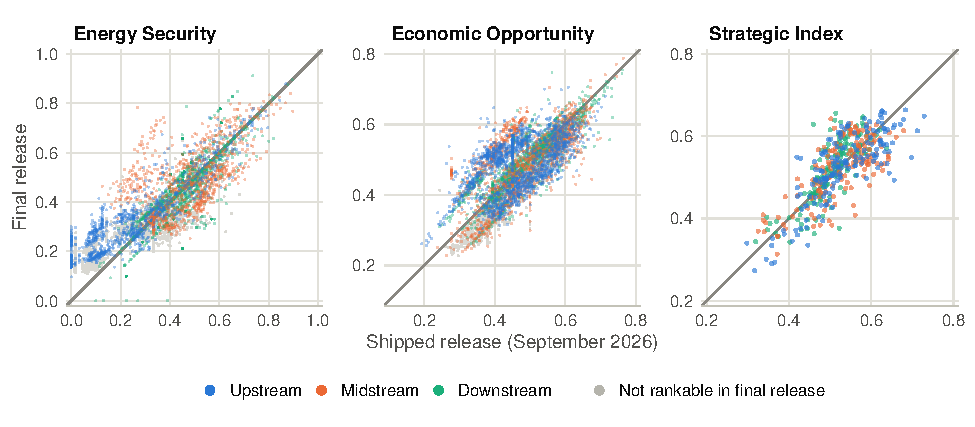
\includegraphics[width=\textwidth]{reconcile_scatter}
  \caption{Shipped against final release, cell by cell. Each point is a country--technology--stage
  cell (Energy Security, Economic Opportunity) or a country--sector cell (Strategic Index) present in
  both releases, with the shipped value (3~September 2026) on the horizontal axis and the final value
  (12~October 2026) on the vertical axis. Colour marks the stage of cells rankable in the final release
  (sovereign economy, at most half of the index weight imputed); grey points are matched cells that
  are not rankable. Energy Security: 5{,}305 matched cells, 3{,}537 rankable; Economic Opportunity:
  6{,}598 and 4{,}290; Strategic Index: the 477 cells of the 18 economies of the shipped hand-picked
  list scored in both releases. Technology--stage pairs in which a pillar is constant in either
  release are excluded. Spearman correlations over rankable cells: 0.81, 0.67 and 0.74. Shipped
  names are mapped to canonical names before matching (item C1). Sources: \texttt{index\_outputs.rds}
  of the two releases; \texttt{scripts/paper/fig\_reconcile.R}.}
  \label{fig:reconcile_scatter}
\end{figure}

A pooled correlation mixes level shifts of whole cells with reorderings within them.
Figure~\ref{fig:reconcile_cells} separates the two. The median within-cell correlation is 0.83 for
$\ES$ and 0.77 for $\EO$; 45 percent of $\ES$ values and 56 percent of $\EO$ values move by more than
ten places in their cell (median moves of 9 and 13 places). A two-factor Shapley decomposition of
each cell's change, with an unobserved shipped category counted as zero at full weight, splits it
into score effects of categories present in both releases and a composition effect from categories
that enter or leave. Composition accounts for 25 percent of the summed absolute change in $\ES$ and
40 percent in $\EO$. When the entering or leaving category is constant within a cell (the zero
Investment cells, Energy Prices, readiness) it moves the cell's level and leaves the ordering
unchanged; the reorderings come from rebuilt inputs, chiefly Foreign Dependency in the $\ES$
Upstream, Trade in the $\ES$ Midstream and Consumption or Investment in the $\ES$ Downstream. The
extreme case is $\EO$ Green Hydrogen Midstream, with a within-cell correlation of $-0.55$: both
releases rank its economies mostly on imputed values, and neither ranking should be read as a
measurement. $\ES$ Nuclear Midstream combines the largest level shift (a mean gain of 0.24, from the
removal of the zero Investment category) with a within-cell correlation of 0.59 (from the rebuilt
Trade category).

\begin{figure}[htbp]
  \centering
  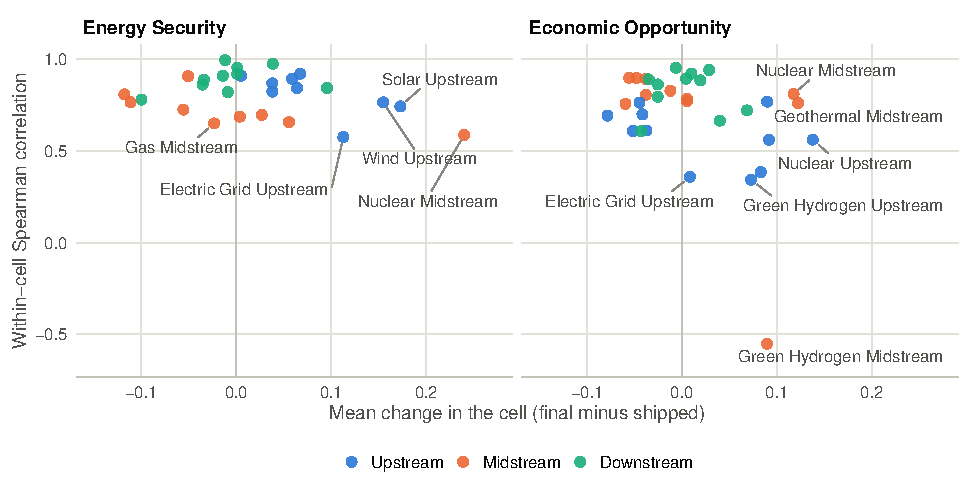
\includegraphics[width=\textwidth]{reconcile_cells}
  \caption{Level shift and rank agreement by technology--stage cell. Each point is one cell.
  Horizontal axis: mean change of the pillar (final minus shipped) across the economies scored in the
  cell in both releases and rankable in the final release. Vertical axis: Spearman correlation of the
  shipped and final values across the same economies. Colour marks the stage; labels name the three
  cells with the lowest correlation and the three with the largest absolute mean change in each panel.
  Energy Security: 28 cells (Nuclear Upstream, constant in the shipped release, is excluded;
  Geothermal Upstream and Midstream and Electric Grid Downstream have no final score; Green Hydrogen
  Midstream had no shipped one); Economic Opportunity: all 33 cells. A point far from zero
  horizontally but high vertically is a level shift that left the ordering largely intact. Sources: as
  in Figure~\ref{fig:reconcile_scatter}.}
  \label{fig:reconcile_cells}
\end{figure}

\paragraph{Coalition members.} Among the 57 members the rankable matched cells number 1{,}468
($\ES$) and 1{,}716 ($\EO$), with correlations of 0.82 and 0.68, close to the full sample.
Figure~\ref{fig:reconcile_movers} and Table~\ref{tab:reconcile_movers} show the twelve largest
changes in each pillar, at most two per cell. The largest are Canada and Namibia in Nuclear Upstream,
from zero to 0.74 and 0.72 in $\ES$: the shipped cell held only the zero Investment category, and the
Red Book places both among the leading holders and producers of uranium. The others trace the
rebuilt themes: consumption (E5), the zero-filled Investment cells (E7), the new Upstream trade
baskets, mirror trade for Gabon, which did not report imports in 2024, and the reviewed copper and
aluminium basket for the United States in Electric Grid Upstream. Eight of the twelve $\ES$ changes
and seven of the twelve $\EO$ changes are mainly composition effects, so they matter most for
comparisons across one country's cells, which is what the Strategic Index makes.

\begin{figure}[htbp]
  \centering
  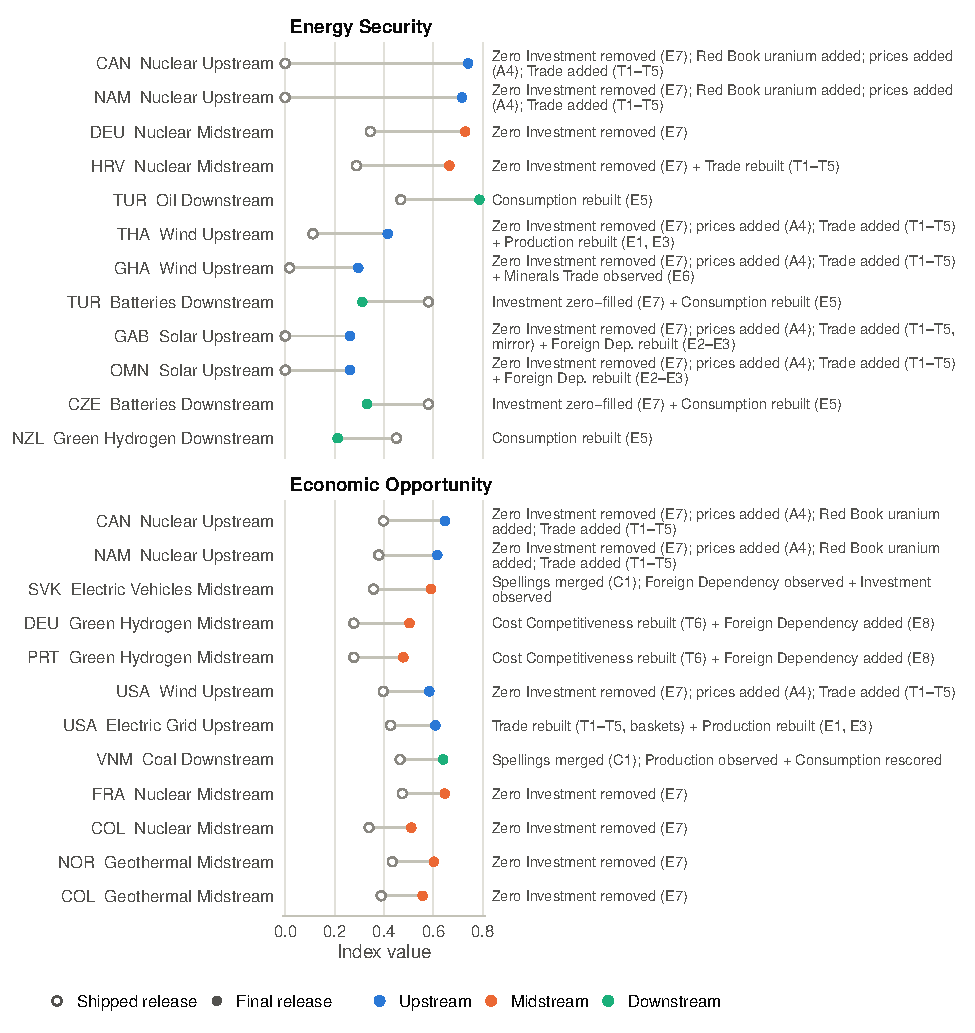
\includegraphics[width=\textwidth]{reconcile_movers}
  \caption{The twelve largest changes among coalition members, by pillar, at most two per
  technology--stage cell. Each row is one member's cell (ISO3 code). Hollow circles mark the shipped
  value and filled circles the final value, coloured by stage. The text at the right names the cause:
  the largest effect in a two-factor Shapley decomposition of the change into category score effects
  and a composition effect (categories entering or leaving and the renormalisation of weights), and
  the second when it is at least half as large, with the data change behind it (``Red Book uranium'':
  OECD-NEA/IAEA resources and production; ``mirror'': trade measured from partners' declarations).
  Item codes refer to Table~\ref{tab:corrections_index}; the full decomposition is in
  Table~\ref{tab:reconcile_movers}. Sample: the 57 members of the final coalition, cells present in
  both releases and rankable in the final release (Energy Security in Nuclear Upstream, constant in the
  shipped release, is included as a mover). Sources: \texttt{category\_contributions} of the two
  \texttt{index\_outputs.rds}.}
  \label{fig:reconcile_movers}
\end{figure}

\begingroup
  \singlespacing\scriptsize
  \setlength{\tabcolsep}{3pt}
  \setlength{\LTcapwidth}{\textwidth}
  \begin{longtable}{@{}>{\raggedright\arraybackslash}p{0.75in} >{\raggedright\arraybackslash}p{0.95in} c c c >{\raggedright\arraybackslash}p{1.05in} >{\raggedright\arraybackslash}p{1.9in}@{}}
  \caption{Largest pillar changes among coalition members and their attribution}
  \label{tab:reconcile_movers}\\
    \toprule
    Member & Cell & Shipped & Final & \makecell{Composition\\effect} & Largest score effect & Attributed cause \\
    \midrule
  \endfirsthead
    \multicolumn{7}{@{}l}{\small\textbf{Table \thetable:} continued}\\
    \toprule
    Member & Cell & Shipped & Final & \makecell{Composition\\effect} & Largest score effect & Attributed cause \\
    \midrule
  \endhead
    \bottomrule
  \endfoot
    \multicolumn{7}{@{}l}{\emph{Energy Security}} \\
    Canada & Nuclear Upstream & 0.000 & 0.741 & +0.741 & -- & Zero Investment cell removed (E7); uranium Reserves and Production added (Red Book); Energy Prices added (A4); Trade added (T1--T5; all-reporter dyads) \\
    Namibia & Nuclear Upstream & 0.000 & 0.716 & +0.716 & -- & Zero Investment cell removed (E7); uranium Reserves and Production added (Red Book); Energy Prices added (A4); Trade added (T1--T5; all-reporter dyads) \\
    Germany & Nuclear Midstream & 0.345 & 0.729 & +0.286 & Trade +0.099 & Zero Investment cell removed (E7) \\
    Croatia & Nuclear Midstream & 0.288 & 0.665 & +0.251 & Trade +0.126 & Zero Investment cell removed (E7) + Trade rebuilt (T1--T5; all-reporter dyads) \\
    Turkiye & Oil Downstream & 0.468 & 0.787 & +0.000 & Consumption +0.320 & Consumption rebuilt (E5) \\
    Thailand & Wind Upstream & 0.112 & 0.415 & +0.127 & Production +0.123 & Zero Investment cell removed (E7); Energy Prices added (A4); Trade added (T1--T5; all-reporter dyads) + Production rebuilt (E1, E3) \\
    Ghana & Wind Upstream & 0.018 & 0.296 & +0.105 & Minerals Trade +0.088 & Zero Investment cell removed (E7); Energy Prices added (A4); Trade added (T1--T5; all-reporter dyads) + Minerals Trade observed, was imputed (E6) \\
    Turkiye & Batteries Downstream & 0.580 & 0.312 & +0.000 & Investment $-$0.165 & Investment zero-filled (E7) + Consumption rebuilt (E5) \\
    Gabon & Solar Upstream & 0.000 & 0.263 & +0.105 & Foreign Dependency +0.086 & Zero Investment cell removed (E7); Energy Prices added (A4); Trade added (T1--T5; all-reporter dyads, mirror imports) + Foreign Dependency rebuilt (E2--E3) \\
    Oman & Solar Upstream & 0.000 & 0.262 & +0.090 & Foreign Dependency +0.086 & Zero Investment cell removed (E7); Energy Prices added (A4); Trade added (T1--T5; all-reporter dyads) + Foreign Dependency rebuilt (E2--E3) \\
    Czech Republic & Batteries Downstream & 0.580 & 0.331 & +0.000 & Investment $-$0.165 & Investment zero-filled (E7) + Consumption rebuilt (E5) \\
    New Zealand & Green Hydrogen Downstream & 0.451 & 0.212 & +0.000 & Consumption $-$0.238 & Consumption rebuilt (E5) \\
    \addlinespace
    \multicolumn{7}{@{}l}{\emph{Economic Opportunity}} \\
    Canada & Nuclear Upstream & 0.398 & 0.647 & +0.266 & Technology Demand $-$0.015 & Zero Investment cell removed (E7); Energy Prices added (A4); Production added (E1, E3; uranium, Red Book); Trade added (T1--T5; all-reporter dyads) \\
    Namibia & Nuclear Upstream & 0.379 & 0.616 & +0.257 & Cost Competitiveness $-$0.016 & Zero Investment cell removed (E7); Energy Prices added (A4); Production added (E1, E3; uranium, Red Book); Trade added (T1--T5; all-reporter dyads) \\
    Slovak Republic & Electric Vehicles Midstream & 0.358 & 0.591 & +0.000 & Foreign Dependency +0.148 & Spellings merged (C1); Foreign Dependency observed + Investment observed \\
    Germany & Green Hydrogen Midstream & 0.278 & 0.503 & +0.066 & Cost Competitiveness +0.098 & Cost Competitiveness rebuilt (T6) + Foreign Dependency added (E8) \\
    Portugal & Green Hydrogen Midstream & 0.278 & 0.479 & +0.070 & Cost Competitiveness +0.118 & Cost Competitiveness rebuilt (T6) + Foreign Dependency added (E8) \\
    United States & Wind Upstream & 0.397 & 0.584 & +0.164 & Production +0.064 & Zero Investment cell removed (E7); Energy Prices added (A4); Trade added (T1--T5; all-reporter dyads) \\
    United States & Electric Grid Upstream & 0.427 & 0.608 & +0.069 & Trade +0.079 & Trade rebuilt (T1--T5; all-reporter dyads, basket review) + Production rebuilt (E1, E3) \\
    Viet Nam & Coal Downstream & 0.465 & 0.640 & +0.000 & Production +0.052 & Spellings merged (C1); Production observed + Consumption rescored \\
    France & Nuclear Midstream & 0.474 & 0.647 & +0.124 & Trade +0.034 & Zero Investment cell removed (E7) \\
    Colombia & Nuclear Midstream & 0.340 & 0.511 & +0.094 & Trade +0.044 & Zero Investment cell removed (E7) \\
    Norway & Geothermal Midstream & 0.434 & 0.602 & +0.148 & Cost Competitiveness +0.038 & Zero Investment cell removed (E7) \\
    Colombia & Geothermal Midstream & 0.389 & 0.557 & +0.134 & Cost Competitiveness +0.050 & Zero Investment cell removed (E7) \\
  \end{longtable}
  \vspace{-6pt}\footnotesize\noindent
    \emph{Notes:} The 12 largest absolute changes, final minus shipped release, of $\ES_{its}$ and of $\EO_{its}$ among the 57 members of the final coalition, at most 2 per technology--stage cell, over the headline cells present in both releases that the final release ranks (sovereign economy, at most half of the index weight imputed); cells that were constant across countries in the shipped release are included. The change is split by a two-factor Shapley decomposition of the weighted category mean: the score effect of a category present in both releases is $\tfrac12(\omega^{\text{shipped}}_k+\omega^{\text{final}}_k)(c^{\text{final}}_k-c^{\text{shipped}}_k)$, with $\omega_k$ the normalised category weight and an unobserved shipped category counted as $c_k=0$ (item A1); the composition effect is the remainder, due to categories that enter or leave and to the renormalisation of the weights. The cause names the largest effect, and the second when it is at least half as large; item codes refer to Table~\ref{tab:corrections_index}. Data changes: ``uranium, Red Book'' = identified recoverable resources and mine production of the OECD-NEA/IAEA Red Book; ``USGS MCS 2026'' = critical-mineral reserves of the USGS Mineral Commodity Summaries 2026; ``all-reporter dyads'' = trade rebuilt from all-reporter Comtrade dyads (importer report first, else the exporter's declaration $\times 1.06$) and the energy-trade file rebuilt from the same pull; ``basket review'' = a stage whose HS6 basket the October 2026 review changed; ``mirror imports'' = an economy that did not report 2024 imports, whose imports come from partners' declarations; ``TRL by stage'' = technology readiness mapped by stage from the IEA Clean Technology Guide. Source: \texttt{category\_contributions} of the two \texttt{index\_outputs.rds}.\par
\endgroup
\medskip


\paragraph{Strategic Index.} The shipped index scored 571 cells of 18 economies of its hand-picked
list; the final one scores 3{,}154 cells of 174 countries in 30 sectors. On the 477 cells scored in
both the correlation is 0.74, and across sectors within a country the median is 0.74 (Argentina 0.42
to Kenya 0.92). The policy term changed most. The shipped Policy index combined IEA PAMS, CAT, the
February 2026 NIPO component and the dual-use score; the final one combines IEA PAMS and CAT, and all
18 economies have both. The within-country policy term correlates only 0.61 between releases and
accounts for 40 percent of the summed absolute change, against 35 percent for security need, 22
percent for $\EO$ and 3 percent for the fixed weights, which differ only through the technology
weights of oil (0.12 shipped, 0 final) and coal (0 and 0.02; item P9). In the final run 215
countries are policy-eligible (65 on IEA PAMS and CAT, 150 on IEA PAMS alone); all 23 economies of
the shipped hand-picked list are among them, as are all 57 members of the derived coalition.
Figure~\ref{fig:reconcile_si_terms} splits the twelve largest changes into their terms. For the final
release Geothermal Midstream is excluded by rule, as before; no sector is constant in either pillar,
because Nuclear Upstream now varies with the Red Book data; and Electric Grid Downstream and
Geothermal Upstream have no $\ES$ value, so the index covers 30 sectors.

\begin{figure}[htbp]
  \centering
  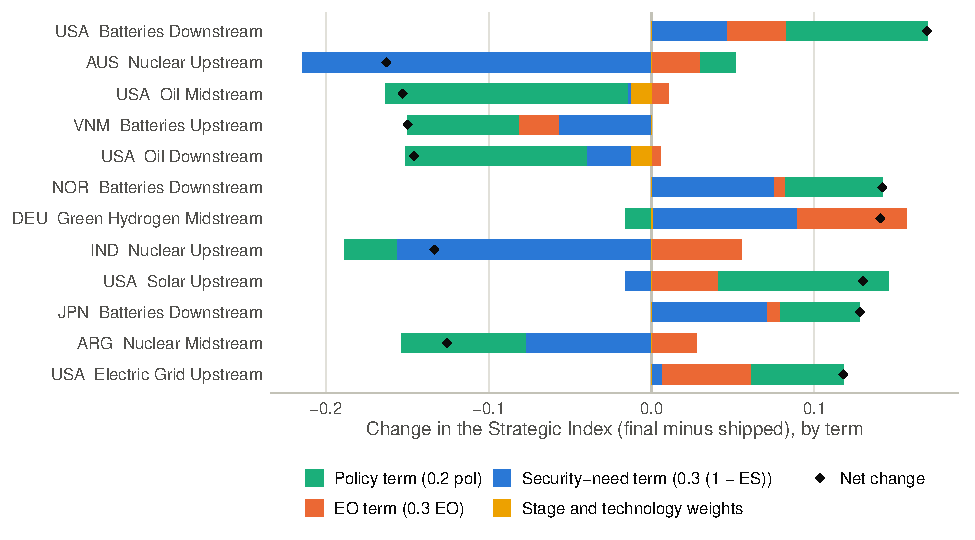
\includegraphics[width=\textwidth]{reconcile_si_terms}
  \caption{The twelve largest changes in the Strategic Index among the economies scored in both
  releases, split into the weighted terms of $\SI=0.2\,\POL+0.3\,\EO+0.3\,(1-\ES)+0.1\,\lambda_s+0.1\,g_t$.
  Each bar is one country--sector cell; the segments are the changes of the policy term, the $\EO$
  term, the security-need term and the two fixed weights combined, and the diamond is the net change,
  which the segments sum to exactly. The shipped policy term is the within-country S-curve of the
  four-component Policy index of February 2026 (IEA PAMS, CAT, NIPO, dual use); the final one is that
  of IEA PAMS and CAT. The policy term is the largest contributor in seven of the twelve, security need
  in five. Sample: the 477 cells of the 18 economies of the shipped hand-picked list scored in both
  releases. Sources: \texttt{strategic\_index} of the two \texttt{index\_outputs.rds};
  \texttt{scripts/paper/fig\_reconcile.R}.}
  \label{fig:reconcile_si_terms}
\end{figure}

\paragraph{The allied picks.} The shipped picks were made over a hand-picked list of 23 economies,
the final ones over the 57 members of the derived coalition, so the comparison covers the 21 they
share (Table~\ref{tab:reconcile_allied}). Kenya and the United Arab Emirates are not members of the
final coalition, and Denmark, France, Italy and South Korea had no shipped pick because they lacked
a Policy index (P3). Of the 17 members with a pick in both releases, 16 change it; only Chile keeps
Nuclear Upstream. Six changes (Australia, Brazil, Canada, India, Mexico and the United States) are
reorderings by the security-need term: all six picked Nuclear Upstream where the shipped $\ES$ was
zero for everyone, and the Red Book now records uranium for all six. Four (Argentina, Indonesia,
South Africa, Viet Nam) are reorderings by the policy term, four (Germany, Japan, Morocco, Norway)
are barred by the endowment screen, and two (Saudi Arabia, the United Kingdom) are no longer scored
because the $\EO$ cell of the shipped pick is not rankable. On these members the picks move from
Nuclear Upstream (8) and Batteries Upstream (5) to Batteries Midstream (13).

\begin{table}[htbp]
  \centering
  \begin{threeparttable}
  \caption{Allied pick per member of the shipped list: shipped and final release}
  \label{tab:reconcile_allied}
  \footnotesize
  \begin{tabularx}{\textwidth}{@{}l >{\raggedright\arraybackslash}p{1.15in} c >{\raggedright\arraybackslash}p{1.15in} c >{\raggedright\arraybackslash}X@{}}
    \toprule
    & \multicolumn{2}{c}{Shipped release} & \multicolumn{2}{c}{Final release} & \\
    \cmidrule(lr){2-3}\cmidrule(lr){4-5}
    Member & Pick & $\SI$ & Pick & $\SI$ & Status or cause of change \\
    \midrule
    Argentina & Electric Vehicles, Midstream & 0.624 & Batteries, Upstream & 0.551 & reordered by the policy term \\
    Australia & Nuclear, Upstream & 0.656 & Batteries, Midstream & 0.610 & reordered by the security-need term \\
    Brazil & Nuclear, Upstream & 0.613 & Batteries, Midstream & 0.606 & reordered by the security-need term \\
    Canada & Nuclear, Upstream & 0.638 & Electric Grid, Midstream & 0.615 & reordered by the security-need term \\
    Chile & Nuclear, Upstream & 0.626 & Nuclear, Upstream & 0.645 & unchanged \\
    Denmark & -- & -- & Batteries, Midstream & 0.636 & new \\
    France & -- & -- & Batteries, Midstream & 0.642 & new \\
    Germany & Batteries, Upstream & 0.712 & Batteries, Midstream & 0.623 & shipped pick screened: no resource base \\
    India & Nuclear, Upstream & 0.643 & Batteries, Midstream & 0.628 & reordered by the security-need term \\
    Indonesia & Electric Vehicles, Midstream & 0.642 & Nuclear, Midstream & 0.568 & reordered by the policy term \\
    Italy & -- & -- & Batteries, Midstream & 0.639 & new \\
    Japan & Batteries, Upstream & 0.657 & Nuclear, Upstream & 0.620 & shipped pick screened: no resource base \\
    Kenya & Batteries, Upstream & 0.701 & \emph{not a member} & -- & not in final coalition \\
    Mexico & Nuclear, Upstream & 0.624 & Batteries, Midstream & 0.564 & reordered by the security-need term \\
    Morocco & Solar, Upstream & 0.683 & Electric Grid, Midstream & 0.609 & shipped pick screened: no resource base \\
    Norway & Nuclear, Upstream & 0.729 & Batteries, Upstream & 0.618 & shipped pick screened: no resource base \\
    Saudi Arabia & Batteries, Upstream & 0.688 & Nuclear, Upstream & 0.567 & shipped pick not scored: EO not rankable \\
    South Africa & Electric Grid, Midstream & 0.679 & Batteries, Midstream & 0.620 & reordered by the policy term \\
    South Korea & -- & -- & Batteries, Midstream & 0.635 & new \\
    United Arab Emirates & -- & -- & \emph{not a member} & -- & not in final coalition \\
    United Kingdom & Batteries, Upstream & 0.690 & Batteries, Midstream & 0.617 & shipped pick not scored: EO not rankable \\
    United States & Nuclear, Upstream & 0.613 & Batteries, Midstream & 0.632 & reordered by the security-need term \\
    Viet Nam & Batteries, Upstream & 0.698 & Batteries, Midstream & 0.606 & reordered by the policy term \\
    \bottomrule
  \end{tabularx}
  \begin{tablenotes}[flushleft]\footnotesize
    \item \emph{Notes:} The pick is the member's Upstream or Midstream sector with the highest Strategic Index; Geothermal and Green Hydrogen are excluded by rule of the selection. Shipped release: the Strategic Index of 3~September 2026 over its hand-picked list of 23 economies, of which 18 had a pick. Final release: \texttt{data/processed/charts/allied\_strategic.csv}, over the derived coalition of 57 members, with the endowment screen (an Upstream extraction stage is eligible only where the member has recorded reserves or production of its resources). The comparison is on the 21 members the two lists share; 2 economies of the shipped list are not in the final coalition. ``new'': a pick only in the final release. Cause of a change: the shipped pick is no longer scored (its exclusion), is barred by the endowment screen, or is outscored, in which case the term of the index that contributes most to the reversal of the two sectors' order is named (an exact split of the reversal into the five weighted terms). The picks of the other 36 final members are reported in Section~\ref{sec:strategic}.
  \end{tablenotes}
  \end{threeparttable}
\end{table}


\paragraph{Network and partnership strength.} The shipped network outputs are not comparable with
the final ones (Table~\ref{tab:reconcile_network}). The shipped diagnostics record a greedy solution
in all 33 stages over 22 effective members, and in 14 stages a producer count of $k^2$ with a
Herfindahl index of one, the signature of \eqref{eq:corr_fanout}; the portfolio loop stopped at its
limit with 12 members above their caps. The final design solves 22 stages over 37 nodes by MILP, with
7 to 10 producers per stage and a median designed Herfindahl index of 0.152, and the loop converges
in seven passes. The shipped release did not write the PSI to disk; reconstructed from the March 2026
partner tables with the shipped logic, it correlates $-0.09$ with the final world view over 187
partners and $-0.33$ with the core view over 191. The denominator defect (B4) placed high-income
partners below the others, so correcting it moves that group up as a block: the United States moves
from 168th to 4th of the 187 in the world view and to 1st in the core view, and Germany from 135th to
5th. China moves from 22nd to 1st in the world view but to 44th in the core view, whose Friendshore
scores rate China from the core members' viewpoints, alignment included.

\begin{table}[htbp]
  \centering
  \begin{threeparttable}
  \caption{Allied network diagnostics: shipped and final release}
  \label{tab:reconcile_network}
  \small
  \begin{tabular}{@{}l c c@{}}
    \toprule
    & Shipped release & Final release \\
    \midrule
    Network nodes & 22 & 37 \\
    Stages designed & 33 (all three stages) & 22 (Upstream, Midstream) \\
    Solver used (stages) & greedy (33) & MILP (22) \\
    Stages with $n_{\text{producers}}=k^2$ and $\HHI=1$ & 14 & 0 \\
    Reported producers per stage & 3--193{,}600 & 7--10 (median 9) \\
    $\HHI$ of designed shares & 0.333--1.000 & 0.126--0.209 (median 0.1520) \\
    Diversification weight $\lambda$ & -- & 0.78 \\
    Policy term in node scores & yes & no \\
    Portfolio loop converged & no & yes \\
    Portfolio passes & 10 (limit) & 7 \\
    Members above their portfolio cap at exit & 12 & 0 \\
    \bottomrule
  \end{tabular}
  \begin{tablenotes}[flushleft]\footnotesize
    \item \emph{Notes:} Shipped release: \texttt{allied\_network\_diagnostics.csv} written on 23~February 2026, the only shipped network artefact read here; it designed every stage of the hand-picked list's 22 effective members (the United Arab Emirates was coded ``UAE'', item N5). In 14 shipped stages a single country was selected with $k^2$ rows of share $1/k$, so the producer count was $k^2$ (with $k$ from 16 to 440) and the Herfindahl index summed over the rows was exactly one (item N1, equation~\eqref{eq:corr_fanout}). Final release: the same file of the final run of 12~October 2026, 37 nodes (the EU-27 as one node), Upstream and Midstream stages only, MILP with the concave diversification term ($\lambda=0.78$, the smallest value on the calibration grid whose median designed $\HHI$ does not exceed the observed one) and portfolio caps, and no policy term in the node scores; the median designed $\HHI$ compares with a median observed export $\HHI$ of the nodes of 0.1556 over the 18 stages with an HS6 basket. The portfolio loop runs over all stages jointly, so it has one outcome per release; the last row counts the members that, when the loop stops, are a top producer in more stages than their cap allows.
  \end{tablenotes}
  \end{threeparttable}
\end{table}


\paragraph{Using numbers from the shipped release.} Within a technology--stage cell, shipped pillar
rankings are a rough guide in the Downstream (median within-cell correlations 0.90 for $\ES$ and 0.88
for $\EO$) and in the $\EO$ Midstream (0.80), a poor guide in the $\ES$ Midstream (0.70) and the $\EO$
Upstream (0.61), and no guide for $\EO$ Green Hydrogen Midstream. Comparisons across cells, and with
them the shipped Strategic Index and its picks, inherit the level shifts and a different Policy index;
the shipped picks should be replaced by those of Section~\ref{sec:strategic}. The shipped network
outputs and any PSI computed from the shipped partner tables should not be used. As the
composite-indicator literature warns, the ordering a composite produces can depend on its
construction as much as on its data \citep{saisana2005uncertainty,saltelli2007composite}; here,
however, the large changes come from defects and new data rather than from defensible alternative
choices, so they are corrections, not a measure of uncertainty.
